\chapter{Derivation of State Machine Models from Process Models\label{chapter:deductive}}

This chapter shows how state machines can be synthesised from process models. They capture the trace semantics of process models, making them amenable to formal analysis such as model-checking.

\section{Motivation and approach\label{section:deductive-motivation}}

Building adequate, complete and consistent process models is not necessarily an easy task. Flawed models can have dreadful consequences in safety-critical areas. The recent usage of process modeling to improve medical safety provides a good example of such area \cite{Clarke:2008, Grando:2009, Damas:2011}; models there should be as error-free as possible. Techniques should therefore be available to support model construction and analysis, in particular for systematically detecting and fixing severe flaws.

A typical analysis technique coming to mind is \emph{model checking} \cite{Clarke:1989}. Model-checking would allow us to verify that a given safety property is satisfied in all process instances. Other kinds of analysis on process models are discussed in \cite{Damas:2011}, including checking the satisfiability of guards; verifying that temporal constraints are met; detecting inaccurate process decisions; and so on. This kind of check should be performed ahead of process enactment.

Verification techniques require a formal semantics for process models. As our guarded hMSCs are an extension of hMSCs, a trace semantics appears natural. This choice also fits the intuition: an event trace can roughly be rephrased in terms of temporal occurrences of tasks. Moreover, a trace semantics for g-hMSCs enables reusing LTS-based tools and techniques \cite{Magee:1999, Giannakopoulou:2003}.

\begin{figure}\centering
\scalebox{0.64}{
  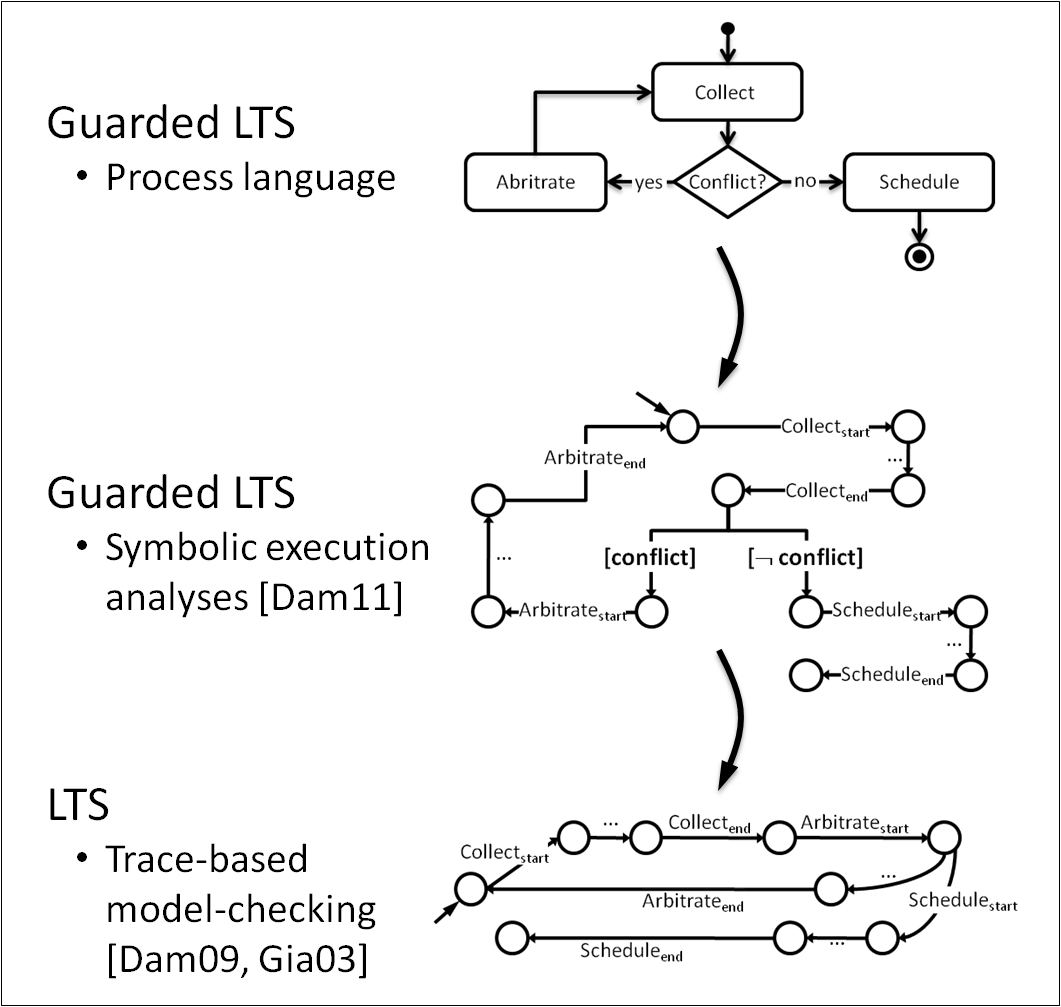
\includegraphics[trim=5mm 2mm 2mm 2mm, clip]{src/3-deductive/images/chapter-overview}
}
\caption{Guarded LTS as an intermediate level between g-hMSC and LTS.\label{image:deductive-chapter-overview}}
\end{figure}

We will only consider the traces of a process globally, that is, as sequences of events seen by an external observer. In other words, in spite of a multi-agent view through message sequence charts, we will not consider agent state machines in isolation. The aim of process modeling is \emph{not} to specify valid executions of the agents themselves, but to capture the control flow of their tasks. 

As a consequence, we will assume a strong sequential composition of g-hMSC nodes and a total ordering of all events inside MSCs (see Section~\ref{subsection:background-hmsc}). In other words, we will assume that agents synchronize with each other when tasks are started and completed. 

To delimit task boundaries in event traces and reason about execution time, each task $T$ will be associated with special events $T_{start}$ and $T_{end}$. These events are assumed to be monitored by all agents; thus, they allow explicitly capturing the required synchronization scheme.

Instead of transforming a guarded hMSC into a LTS directly, we will generate an intermediate form called guarded labeled transition systems (g-LTS). Roughly, a g-LTS is a transition system with guards or events on transitions. It is a structured form of LTS aimed to avoid state explosion. This intermediate form is therefore easier to understand and supports different types of analysis at an abstract level; it may also facilitate code generation for process enactment. 

Figure~\ref{image:deductive-chapter-overview} illustrates the three abstraction levels provided by g-hMSC, g-LTS and LTS, respectively. Analyses about guards, temporal constraints and the like are performed at the g-LTS level. They rely on a generalization of the symbolic execution algorithm used to decorate a LTS with assertions on fluents (see Section \ref{section:background-fluents}). For details about such analyses at the g-LTS level, see \cite{Damas:2011}. Trace-based model-checking can be performed at the LTS level, using slight adaptations of existing tools such as LTSA \cite{Magee:1999} (see Section \ref{section:tool-model-checker}).

Our two derivation algorithms for transforming a guarded hMSC to a guarded LTS then to a LTS are detailed in Section \ref{section:deductive-glts-to-lts}. Section \ref{section:deductive-glts} first introduces guarded LTS formally; it also provides a few operators for manipulating them.

\section{Introducing guarded transition systems\label{section:deductive-glts}}

This section introduces guarded LTS (g-LTS) as an intermediate formalism between guarded hMSCs and LTS. Roughly, a g-LTS is a transition system with guards or events on transitions. It provides a convenient milestone on the way from a guarded hMSC to the corresponding LTS, in particular, for determining the set of traces accepted by the guarded hMSC. As a structured form of LTS, a g-LTS representation avoids state explosion. It is easier to understand and facilitates code generation. Moreover, interresting analyses may be performed at g-LTS level, see \cite{Damas:2011}.

\begin{definition}[Guarded LTS]
\noindent A guarded LTS is defined as a structure $(Q,\Sigma,\Phi,\delta,q_{0},C_{0})$ where 
\begin{itemize}
\item $Q$ is a finite set of states,
\item $\Sigma$ is a set of event labels, 
\item $\Phi$ is a set of fluents defined on $\Sigma$,
\item $\delta$ is a transition relation $Q \times \Sigma_{\tau}\cup\mathcal{P}(2^\Phi) \times Q$,
\item $q_{0} \in Q$ is the initial state,
\item $C_{0} \in \mathcal{P}(2^\Phi)$ is an initial condition. 
\end{itemize}
\end{definition}

In a guarded LTS, transitions are labeled either by a guard or by an event. Non-observable $\tau$-transitions are also allowed; their usage is the same as in pure LTS. 

A guard is a propositional formula over fluents in $\Phi$. The set of such formula is denoted by $\mathcal{P}(2^\Phi)$, as in Section \ref{section:background-fluents}. Intuitively, the guard must be evaluated to true for its transition to be activated. This is made precise is the next section.

The condition $C_0$ plays the same role as in guarded hMSCs. It is a boolean formula that constraints the acceptable initial values of fluents. 

\subsection{Trace semantics\label{subsection:glts-trace-semantics}} 

The semantics of g-LTS is defined in terms of event traces involving no guards at all.

\begin{definition}[g-LTS execution]
An \emph{execution} of a g-LTS $G = (Q,\Sigma,\Phi,\\\delta,q_{0},C_{0})$ from $q_0$ is a pair $(Init, \textless l_0, \ldots,l_n\textgreater)$, where 
\begin{itemize}
\item $Init \in 2^\Phi$ is an initial fluent value assignment, mapping every fluent in $\Phi$ to true or false,
\item $\textless l_0,\ldots,l_n \textgreater$ is an finite sequence of labels $l_i \in \Sigma_{\tau}\cup\mathcal{P}(2^\Phi)$, some of them being event labels (including $\tau$) and others being guards.
\end{itemize}
\end{definition}

Only certain executions are considered valid from the initial state of the g-LTS. This is captured by the following definition:

\begin{definition}[Valid g-LTS execution]
An execution $S = (Init,\textless l_0,\ldots,l_n\textgreater)$ of a g-LTS $G = (Q,\Sigma,\Phi,\delta,q_{0},C_{0})$ is \emph{valid} from its initial state $q_0$ iif the following \emph{acceptance conditions} are met for every $i$ such that $0 \leqslant i < n$:\\
\vspace{-0.8cm}
\begin{tabbing}
\indent trace inclusion:~~~~~~~\= $\exists q_{i+1} \in Q$ such that $(q_i,l_i,q_{i+1}) \in \delta$\\
\indent admissible start:      \> $Init \models C_0$ \\
\indent guard satisfaction:    \> $S_i \models l_i$ if $l_i \in \mathcal{P}(2^\Phi)$\\
\end{tabbing}
\vspace{-0.8cm}
where $S_i$ is the fluent value assignment after the i-th event in the trace, with $S_0 = Init$.
\end{definition}

The first condition states that the label sequence denotes an existing path in the automaton. The second condition states that the initial fluent value assignment must meet the initial condition $C_0$. The third condition ensures that all guards are met along the sequence.

The trace semantics of a g-LTS is defined as a set of event traces. Roughly, it consists of all valid executions where $\tau$ labels as well as guards have been removed. This is precisely captured by the the following definition.

\begin{definition}[g-LTS trace semantics]
The set of traces accepted by a g-LTS $G = (Q,\Sigma,\Phi,\delta,q_{0},C_{0})$ is defined as:
\begin{align*}
\mathcal{L}(G) &= \{~w|_{\Sigma} \mid \exists~Init \in 2^\Phi~s.t.~(Init,w)~is~a~valid~execution~for~G~\}
\end{align*}
\end{definition}

Section \ref{subsection:from-glts-to-lts} provides a composition algorithm to capture this set of traces through a pure LTS, that is, a LTS with event labels only. The next section will first refine the LTS hiding and composition operators defined in Section \ref{section:background-state-machines} to handle guards.

\subsection{Hiding and composition in presence of guards}

The hiding operator on g-LTSs is very similar to the one on LTSs, defined in Section \ref{subsection:lts-hiding}. 

\begin{definition}[g-LTS hiding]
The \emph{hiding} of a set of labels $I$ in a g-LTS $G = (Q,\Sigma,\Phi,\delta,q_{0},C_{0})$ defines the g-LTS
\begin{equation*}
G \setminus I = (Q,\Sigma \setminus I,\Phi,\delta_{hidden},q_{0},C_0)
\end{equation*}
\noindent where $\delta_{hidden}$ is the smallest relation satisfying the following rules:
\begin{center}
\begin{tabular}{cc}
$\frac{\displaystyle G \stackrel{l}{\longrightarrow} G'}{\displaystyle G \setminus I \stackrel{l}{\longrightarrow} G' \setminus I}~~l \notin I$ & 
$\frac{\displaystyle G \stackrel{l}{\longrightarrow} G'}{\displaystyle G \setminus I \stackrel{\tau}{\longrightarrow} G' \setminus I}~~l \in I$ \\
\end{tabular}
\end{center}
\end{definition}

As with LTSs, the hiding operator makes a set of labels invisible by replacing them by $\tau$ transitions. Note that the definition above allows hiding both guards and events. 

The special case where $I = \mathcal{P}(2^\Phi)$ yields a g-LTS with no guard remaining. In this case, we will consider that the hiding operator actually returns a LTS defined as follows:
\begin{equation*}
G \setminus \mathcal{P}(2^\Phi) = (Q,\Sigma,\delta_{hidden},q_0)
\end{equation*}

We also define a composition operator on g-LTS, as follows:

\begin{definition}[g-LTS composition]
Let $G = (Q_1,\Sigma_1,\Phi_1,\delta_1,q_{1},C_{1})$ and $H = (Q_2,\Sigma_2,\Phi_2,\delta_2,q_{2},C_{2})$ denote two g-LTS. Their \emph{composition} is another g-LTS 
\begin{equation*}
G \parallel H = (S_1 \times S_2,\Sigma_1\cup\Sigma_2,\Phi_1\cup\Phi_2,\delta,(q_1,q_2),C_1 \wedge C_2)
\end{equation*}
\noindent where $\delta$ is the smallest relation satisfying the following rules:

\centering
\begin{tabular}{cl}
$\frac{\displaystyle G \stackrel{l}{\longrightarrow} G'}{\displaystyle G \parallel H \stackrel{l}{\longrightarrow} G' \parallel H}$ & $l \notin \mathcal{P}(2^\Phi)$, $l \notin \Sigma_2$ \\[20pt]

$\frac{\displaystyle H \stackrel{l}{\longrightarrow} H'}{\displaystyle G \parallel H \stackrel{l}{\longrightarrow} G \parallel H'}$ & $l \notin \mathcal{P}(2^\Phi)$, $l \notin \Sigma_1$ \\[20pt]

$\frac{\displaystyle G \stackrel{l}{\longrightarrow} G',~H \stackrel{l}{\longrightarrow} H'}{\displaystyle G \parallel H \stackrel{l}{\longrightarrow} G' \parallel H'}$ & $l \notin \mathcal{P}(2^\Phi)$, $l \neq \tau$ \\[20pt]

$\frac{\displaystyle G \stackrel{g}{\longrightarrow} G',~H \stackrel{h}{\longrightarrow} H'}{\displaystyle G \parallel H \stackrel{g \wedge h}{\longrightarrow} G' \parallel H'}$ & $g \in \mathcal{P}(2^{\Phi_1})$, $h \in \mathcal{P}(2^{\Phi_2})$, $g \wedge h \nvDash false$ 
\end{tabular}
\end{definition}

The first three rules are the same as with LTS composition (see Section \ref{subsection:lts-composition}); they explicitly exclude guards here. The last rule states that the two LTSs must transit on guards together, provided that their conjunction is satisfiable. The resulting transition is then labeled with this conjunction.


\section{From guarded hMSC to pure LTS\label{section:deductive-glts-to-lts}}

This section presents algorithms for explicitly capturing the traces of a g-hMSC through a pure LTS. Section \ref{subsection:from-ghmsc-to-glts} provides an algorithm for transforming a g-hMSC into a g-LTS. Section \ref{subsection:from-glts-to-lts} then shows that the set of event traces admitted by a g-LTS can be captured through a LTS.

\subsection{From guarded hMSC to guarded LTS\label{subsection:from-ghmsc-to-glts}}

A g-hMSC can be transformed into an equivalent g-LTS. The latter abstracts from the agents and captures the set of global behaviors covered by the g-hMSC. The transformation algorithm extends the technique introduced in Section \ref{subsection:background-hmsc} to synthesize a LTS capturing hMSC traces \cite{Uchitel:2004}. 

\noindent \textbf{Handling nodes} -- Every g-hMSC node yields a behaviorally equivalent sub-LTS (see dashed rectangles at bottom of Fig~\ref{image:scheduler-ghmsc-glts}).
\begin{enumerate}[(a)]
\item A terminal MSC node is transformed into a sub-LTS collecting the linear event sequence from the scenario. For a MSC $M$, the LTS captures the set of traces $\mathcal{L}_{total}(M)$ defined in Section \ref{subsection:background-positive-scenarios}.
\item For a node expanded into a finer-grained g-hMSC, the procedure is applied recursively to obtain the corresponding sub-LTS.
\item A decision node is rewritten as a sub-LTS reduced to one simple state and no event. The same applies to the \emph{start} and \emph{end} nodes of the g-hMSC.
\end{enumerate}

In cases (a) and (b), the special events $\mbox{\emph{Task}}_{start}$ and $\mbox{\emph{Task}}_{end}$ are added as first and last events of the corresponding sub-LTS, respectively.

\begin{figure}[H]
\centering
\scalebox{0.60}{
  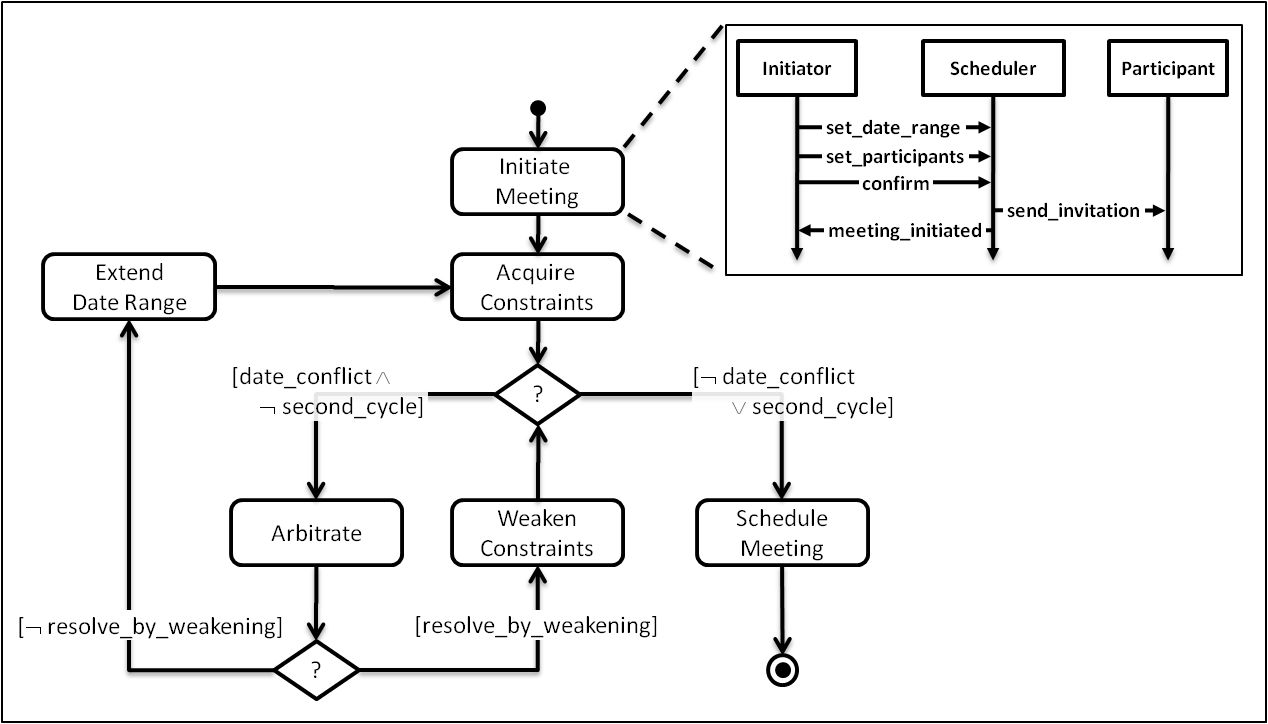
\includegraphics[trim=2mm 2mm 2mm 2mm, clip]{src/2-framework/images/scheduler-ghmsc}
}
\scalebox{0.57}{
  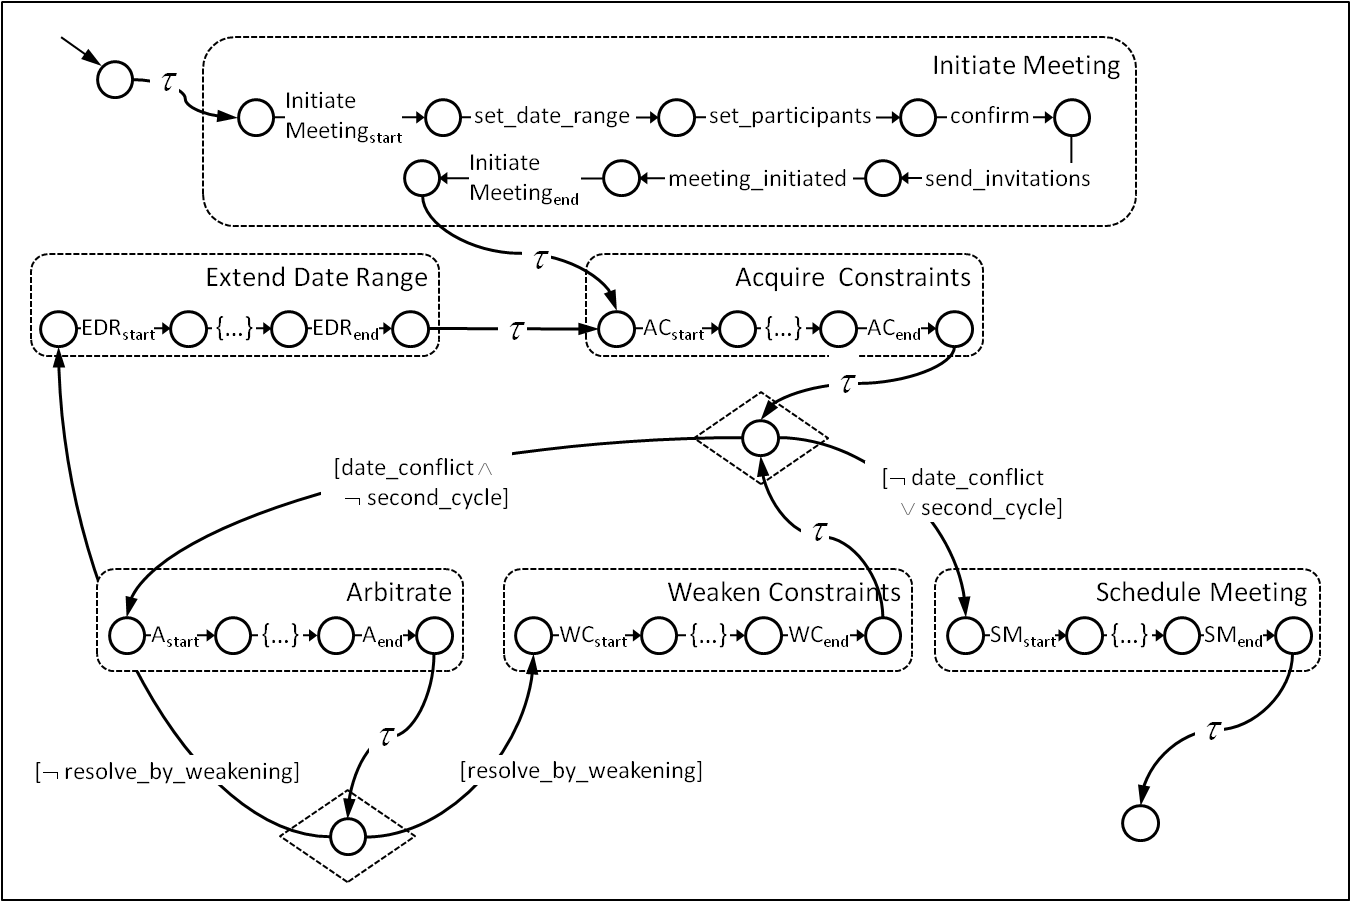
\includegraphics[trim=2mm 2mm 2mm 2mm, clip]{src/3-deductive/images/ghmsc-glts-scheduler}
}
\caption[Transforming a g-hMSC into a g-LTS: the meeting scheduler example]{Transforming a g-hMSC (top) into a g-LTS (bottom): the meeting scheduler example\label{image:scheduler-ghmsc-glts}}
\end{figure}

\noindent \textbf{Handling edges} -- The edges in the g-hMSC yield transitions between the \emph{terminal} and \emph{initial} states of the sub-LTS corresponding to their \emph{source} and \emph{target} nodes, respectively.
\begin{itemize}
\item An outgoing edge of a decision node is further labeled by the corresponding guard to yield a guarded transition in the g-LTS.
\item Any other edge is simply converted to a $\tau$ transition.
\end{itemize}

Fig.~\ref{image:scheduler-ghmsc-glts} illustrates the transformation on the meeting scheduling process. The g-hMSC on top yields the g-LTS at the bottom.
\begin{itemize}
\item In the g-LTS, task ``boundaries'' are kept visible through dashed rectangles surrounding the different sub-LTS.  Similarly, dashed diamonds show which g-LTS states come from decision nodes. 
\item The task \emph{Initiate Meeting} is converted into a sub-LTS capturing the linear event sequence defined by its MSC. This sequence is extended with the special events $\mbox{\emph{InitiateMeeting}}_{start}$ and $\mbox{\emph{InitiateMeeting}}_{end}$.
\item Converting the other tasks is similar, the algorithm being applied recursively on finer-grained g-hMSC. The figure shows that \emph{start} and \emph{end} events are introduced for each of those tasks as well. 
\item Last, outgoing edges of decision nodes lead to guarded transitions in the g-LTS whereas other edges of the g-hMSC yield $\tau$ transitions.
\end{itemize}

The resulting g-LTS can be further optimized by coalescing states separated by $\tau$ transitions, provided the target state has no other incoming transition. The g-LTS state space is thereby reduced; this will speed up the synthesis of a trace-equivalent LTS and the model-checking procedure described in Section \ref{section:tool-model-checker}. 

%However, such optimization breaks the traceability between g-hMSC tasks and g-LTS states. Such traceability turn to be useful in practice for providing users with feedback on the submitted process model itself (see Section \ref{section:tool-clinical-pathway-analyzer}). 

\subsection{From guarded LTS to pure LTS\label{subsection:from-glts-to-lts}}

The set of traces accepted by a g-LTS $G$ may now be captured by a trace-equivalent LTS. There are two steps.
\begin{enumerate}[(1)]
\item First, a parallel composition of g-LTSs is computed so as to meet the various acceptance conditions from Definition \ref{definition:valid-glts-execution} (valid g-LTS execution).
\begin{itemize}
\item The first automaton in this composition is a super g-LTS built from $G$ to initially meet the \emph{trace inclusion} and \emph{admissible start} conditions. This g-LTS actually covers a superset of all admissible event traces and will therefore be pruned.
\item To meet the \emph{guard satisfaction} condition, the set of traces of the super g-LTS is pruned further by composing it with fluent automata, one for each fluent.
\end{itemize}
\item By construction, all paths admitted by the g-LTS resulting from step~(1) yield valid executions for the initial g-LTS $G$. Therefore, guards and $\tau$-transitions can be safely hidden to obtain a pure LTS; the latter captures all event traces of the trace semantics given in Definition~\ref{definition:glts-trace-semantics}.
\end{enumerate}

Let us make each g-LTS in the composition further precise. In the sequel, $G = (Q,\Sigma,\Phi,\delta,q_{0},C_{0})$ will denote the input g-LTS which is transformed to a pure LTS, e.g. the one of Fig.~\ref{image:scheduler-ghmsc-glts}. 

\subsubsection*{Super g-LTS}

By definition, the input g-LTS $G$ already meets the \emph{trace inclusion} condition: the latter simply requires executions to correspond to existing paths in the g-LTS.

In order to meet the \emph{admissible start} condition, $G$ is extended by converting its initial condition $C_0$ into an explicit guard from a new initial state. More precisely, the super g-LTS is defined by:
\begin{equation*}
Super~LTS = (Q \cup \{ q_{start} \}, \Sigma, \Phi, \delta \cup \{(q_{start},C_0,q_0)\},q_{start},true)
\end{equation*}

\begin{figure}[H]
\centering
\scalebox{0.60}{
  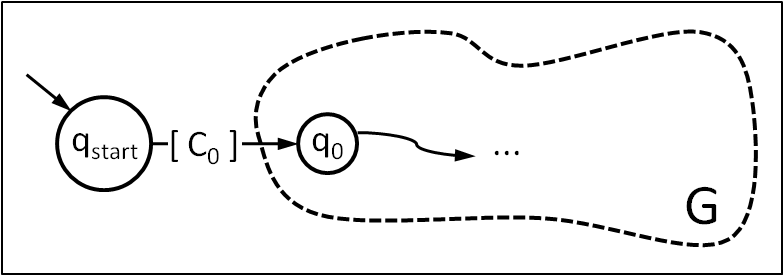
\includegraphics[trim=2mm 2mm 2mm 2mm, clip]{src/3-deductive/images/super-lts}
}
\caption{The super g-LTS\label{image:super-lts}}
\end{figure}

The super g-LTS is illustrated in Fig~\ref{image:super-lts}. The cloud at there simply denotes the g-LTS $G$ taken as input. A guarded transition labeled by $C_0$ reaches its initial state $q_0$ from a newly introduced one $q_{start}$.

During composition, the introduced guarded transition will synchronize with similar guarded transitions in the fluent automata introduced hereafter. Doing so will prune initial fluent assignments that do not satisfy $C_0$. This will guarantee the satisfaction of the \emph{admissible start} condition in a way similar to the satisfaction of guards (see below).

\subsubsection*{Fluent g-LTS}

The \emph{guard satisfaction} condition is enforced by pruning all traces violating guards in the super g-LTS. For this, the super g-LTS is composed with fluent automata that keep track of current fluent values and constrain guards accordingly. Recall that fluents have undertermined initial values; process models and guarded LTS have an initial condition $C_0$ that constrains their values in the initial state. 

Every fluent $Fl = \textless Init_{Fl}, Term_{Fl} \textgreater $ yields a g-LTS $(Q,\Sigma,\Phi,\delta,q_{0},C_{0})$ where:
\begin{align*}
Q      &= \{q_u,q_t,q_f\}            \\
\Sigma &= Init_{Fl} \cup Term_{Fl}   \\
\Phi   &= \{ Fl \} \\
\delta &=    \{~(q_f,e,q_t) \mid e \in Init_{Fl}~\}~\cup \{~(q_t,e,q_t) \mid e \in Init_{Fl}~\} \\
       &\cup~\{~(q_t,e,q_f) \mid e \in Term_{Fl}~\} \cup \{~(q_f,e,q_f) \mid e \in Term_{Fl}~\} \\
       &\cup~\{~(q_u, [Fl], q_t),~(q_u, [\neg Fl], q_f)~\} \\
       &\cup~\{~(q_t, [Fl], q_t),~(q_f, [\neg Fl], q_f)~\} \\
q_0    &= q_u \\
C_0    &= true
\end{align*}

In this definition, $q_u$, $q_t$ and $q_f$ denote g-LTS states where the fluent is \emph{unassigned}, \emph{true} and \emph{false}, respectively (see Fig.~\ref{image:fluent-glts}).
\begin{itemize}
\item The unassigned state $q_u$ is the initial g-LTS state. From there, the \emph{true} and \emph{false} states may be reached through guarded transitions that force the fluent to an initial value consistent with the reached state. These guards will synchronize with the transition labeled by $C_0$ in the super g-LTS, thereby meeting the \emph{admissible start} condition.
\item A fluent g-LTS may transit from its \emph{false} state $q_f$ to its \emph{true} state $q_t$ with the occurrence of events belonging to $Init_{Fl}$ and vice-versa, with events belonging to $Term_{Fl}$. In Fig.~\ref{image:fluent-glts}, a transition labeled with a set between brackets is a shortcut denoting one transition for each element of the set.
\item In each state $q_f$ and $q_t$, a self-looping guard constrains the fluent value to the one denoted by the corresponding state. The conjunction of such guards with the ones of the super g-LTS will force the resulting composition to meet the \emph{guard satisfaction} condition. Indeed, the g-LTS composition operator prunes the conjunctions of guards that are unsatisfiable (see Definition~\ref{definition:glts-composition}).
\item The remaining self-looping transitions labeled with \emph{Init$_{Fl}$} (resp. \\ \emph{Term$_{Fl}$}) from states $q_t$ (resp. $q_f$) is added to avoid over-constraining the composition. That is, initiating (resp. terminating) events may occur even when the fluent is already \emph{true} (resp. \emph{false}).
\end{itemize}

\begin{figure}\centering
\scalebox{0.75}{
  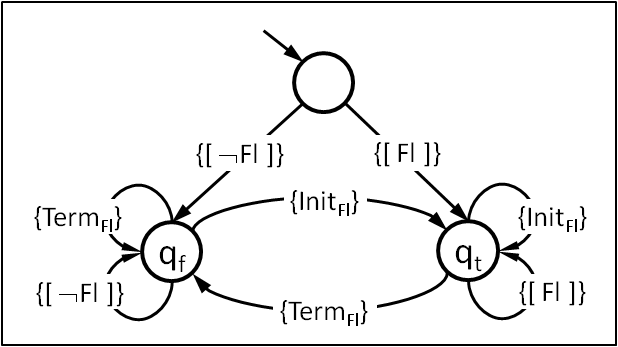
\includegraphics[trim=2mm 2mm 2mm 2mm, clip]{src/3-deductive/images/fluent-glts}
}
\caption{A generic fluent g-LTS\label{image:fluent-glts}}
\end{figure}

For example, consider the following fluent for the meeting scheduler exemplar:
\begin{center}
fluent $second\_cycle = \newline \textless \{ ExtendDateRange_{end}, WeakenConstraints_{end} \}, \newline
 \{ InitiateMeeting_{end} \} \textgreater $\\
\end{center}

The corresponding fluent automaton is shown in Fig.~\ref{image:second-cycle-fluent-glts}.

\begin{figure}\centering
\scalebox{0.75}{
  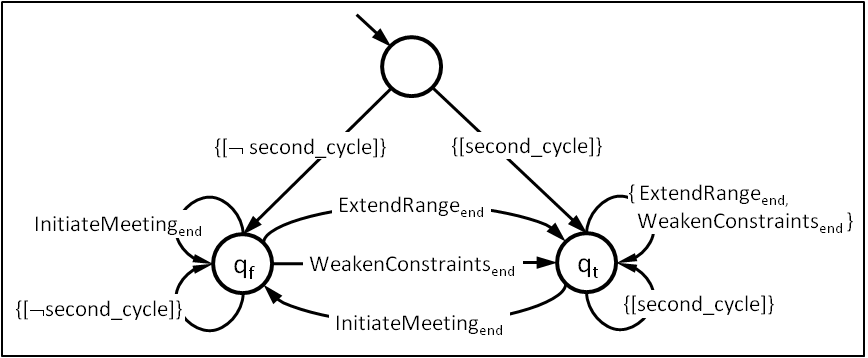
\includegraphics[trim=2mm 2mm 2mm 2mm, clip]{src/3-deductive/images/second-cycle-fluent-glts}
}
\caption{Fluent g-LTS for $second\_cycle$\label{image:second-cycle-fluent-glts}}
\end{figure}

\subsubsection*{Composition automata and hiding guard/$\tau$ labels}

Putting pieces together, the trace-equivalent LTS of a g-LTS is obtained through the following computation:
\begin{align*}
&Composition = (Super~LTS \parallel Fl_1 \parallel \ldots \parallel Fl_n)\\
&Traces      = Composition \setminus \mathcal{P}(2^\Phi),
\end{align*}
where $Fl_i$ denotes the fluent automaton of the i-th fluent.

The first step simply computes the parallel composition of the Super LTS with fluent automata. All guards are then removed from the results through g-LTS hiding, yielding a pure LTS (see Definition~\ref{definition:glts-hiding}). This LTS may be further simplified by removing $\tau$ transitions and minimizing it under trace equivalence (see Section~\ref{section:background-state-machines}).

\begin{figure}
\centering
\scalebox{0.57}{
  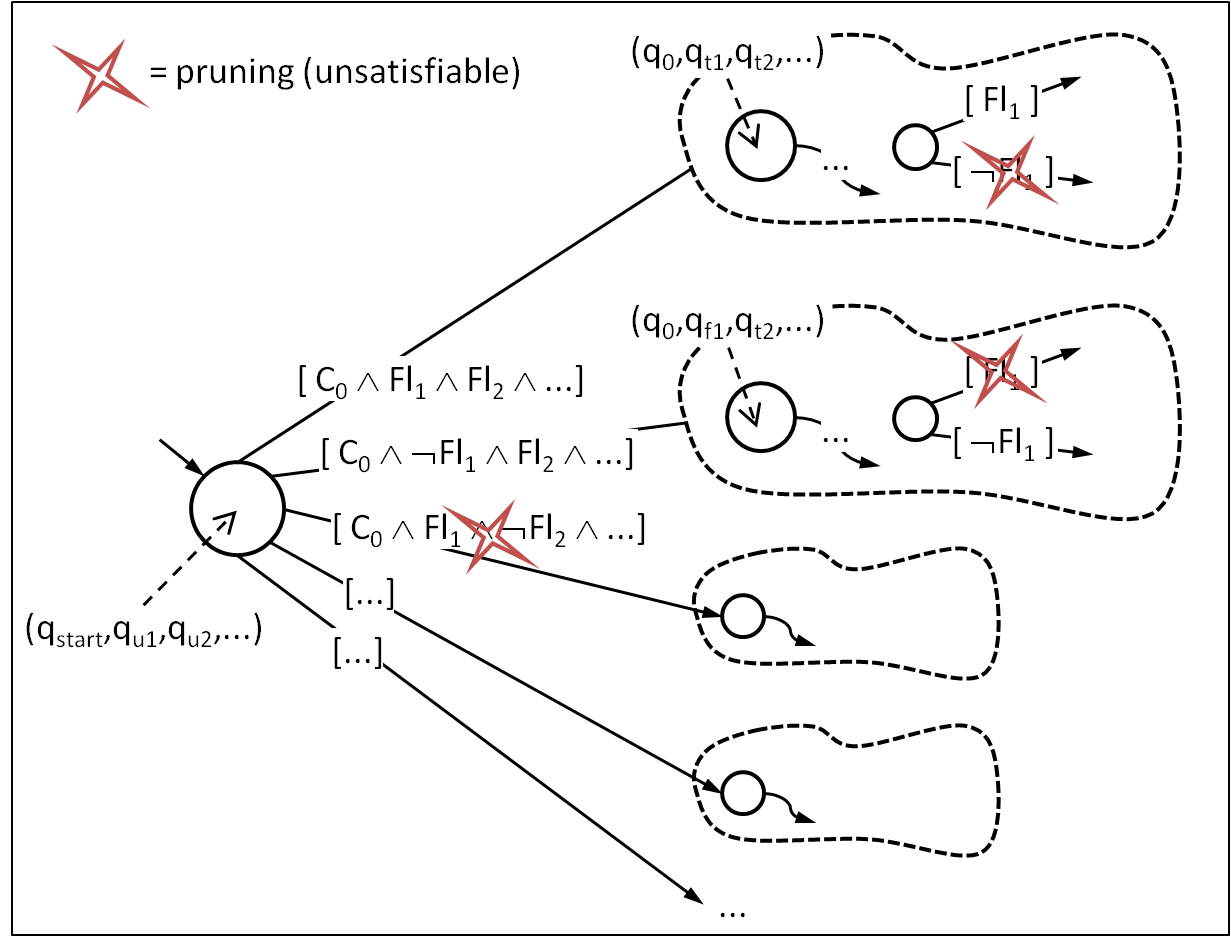
\includegraphics[trim=4mm 2mm 2mm 2mm, clip]{src/3-deductive/images/glts2lts-intuition}
}
\caption{Principle of the composition algorithm for computing the valid traces of a g-LTS.\label{image:glts2lts-intuition}}
\end{figure}

\subsubsection*{Correctness of the synthesis}

The principle of the synthesis algorithm is illustrated in Fig.~\ref{image:glts2lts-intuition}, showing the g-LTS obtained when composing the super g-LTS with fluent automata:
\begin{itemize}
\item From the compound initial state, up to $2^{\mid\Phi\mid}$ guarded transitions may appear. They actually correspond to all possible fluent assignments satisfying $C_0$. Unsatisfiable conjunctions are automatically pruned by the g-LTS composition operator (see Definition \ref{definition:glts-composition}).
\item Each of these transitions leads to a new compound state, namely $q_0$ on the super g-LTS side and $q_t$ or $q_f$ for each fluent automaton, according to the initial fluent assignment reaching the compound state.
\item From every such state, the input g-LTS $G$ is systematically explored; unsatisfiable guards are pruned according to the current fluent values. The latter are tracked by fluent automata that transit from $q_f$ to $q_t$ with the occurrence of initiating and terminating events.
\end{itemize}

Admissible paths from the initial state of such automaton yield sequences of transition labels of the following form:
\begin{align*}\textless g_0~l_0~l_1~l_2~l_3~\ldots~l_n \textgreater \end{align*}
where $g_0$ is a guard and $l_i$ is either a guard or an event label. By construction, $g_0$ actually reduces to a fluent value assignment, that is, a Boolean guard with only one admissible value assignment. Therefore, such sequences denote g-LTS executions (see Definition~\ref{definition:glts-execution}).

We can now show that these executions are valid g-LTS executions for the input g-LTS $G$ (see Definition~\ref{definition:valid-glts-execution}):
\begin{itemize}
\item The \emph{trace inclusion} condition is met since the sub-sequence $\textless l_0~\ldots~l_n \textgreater$ denotes an existing path in $G$. In particular, fluent automata can only prune guards; they could not add behaviors to those already admissible by the input g-LTS.
\item The \emph{admissible start} condition is also met since $g_0$ has been shown to satisfy $C_0$.
\item The \emph{admissible guards} condition is met since unsatisfiable guards are systematically pruned during composition.
\end{itemize}

The \emph{hiding} step removes all guards, yielding a pure LTS that precisely captures the trace semantics from Definition \ref{definition:glts-trace-semantics}. 

In practice, it is convenient to enhance the \emph{hiding} step so as to preserve the initial fluent value assignments $g_0$ labeling the transitions issued of the initial g-LTS state. This amounts capturing the set of valid g-LTS traces from Definition~\ref{definition:valid-glts-traces}. Doing so allows providing the user with a better feedback when using the synthesis algorithm for model-checking g-hMSC and g-LTS (see Section~\ref{section:tool-model-checker}).

\subsubsection*{Example}

Figure~\ref{image:scheduler-lts} shows the resulting LTS obtained on the meeting scheduling example from Fig.~\ref{image:scheduler-ghmsc-glts}. The task refinements are not entirely unfolded there; only events used in fluent definitions were kept.
\begin{itemize}
\item The \emph{no\_remaining\_solution} event, for example, denotes an initiating event of the \emph{date\_conflict} fluent; it belongs to the refinement of the \emph{AcquireConstraints} task. 
\item The events \emph{click\_extend} and \emph{click\_weaken} suggest buttons allowing the meeting initiator to select resolution heuristics when a conflict occurs. They appear in the definition of the fluent \emph{resolve\_by\_weakening}. 
\item A transition labeled with `$\ldots$' denotes a sequence of events not shown for readability.
\end{itemize}

Unlike the original g-hMSC and its g-LTS reformulation, this LTS does not contain any loop. This happens because the $second\_cycle$ fluent prevents indefinite meeting arbitration. In other words, in our example the technique unfolds the process models into three possible scenarios. 
\begin{itemize}
\item In the rightmost one, no date conflict arises and the meeting is scheduled immediately after having acquired the constraints. 
\item In the middle one, a conflict occurs and is resolved by weakening the participant constraints. 
\item In the leftmost one, the resolution consists in extending the date range and collecting constraints one again. \item In the last two cases, even if the absence of an optimal solution triggers a new date conflict, the meeting is scheduled. 
\end{itemize}

\begin{figure}
\centering
\scalebox{0.15}{
  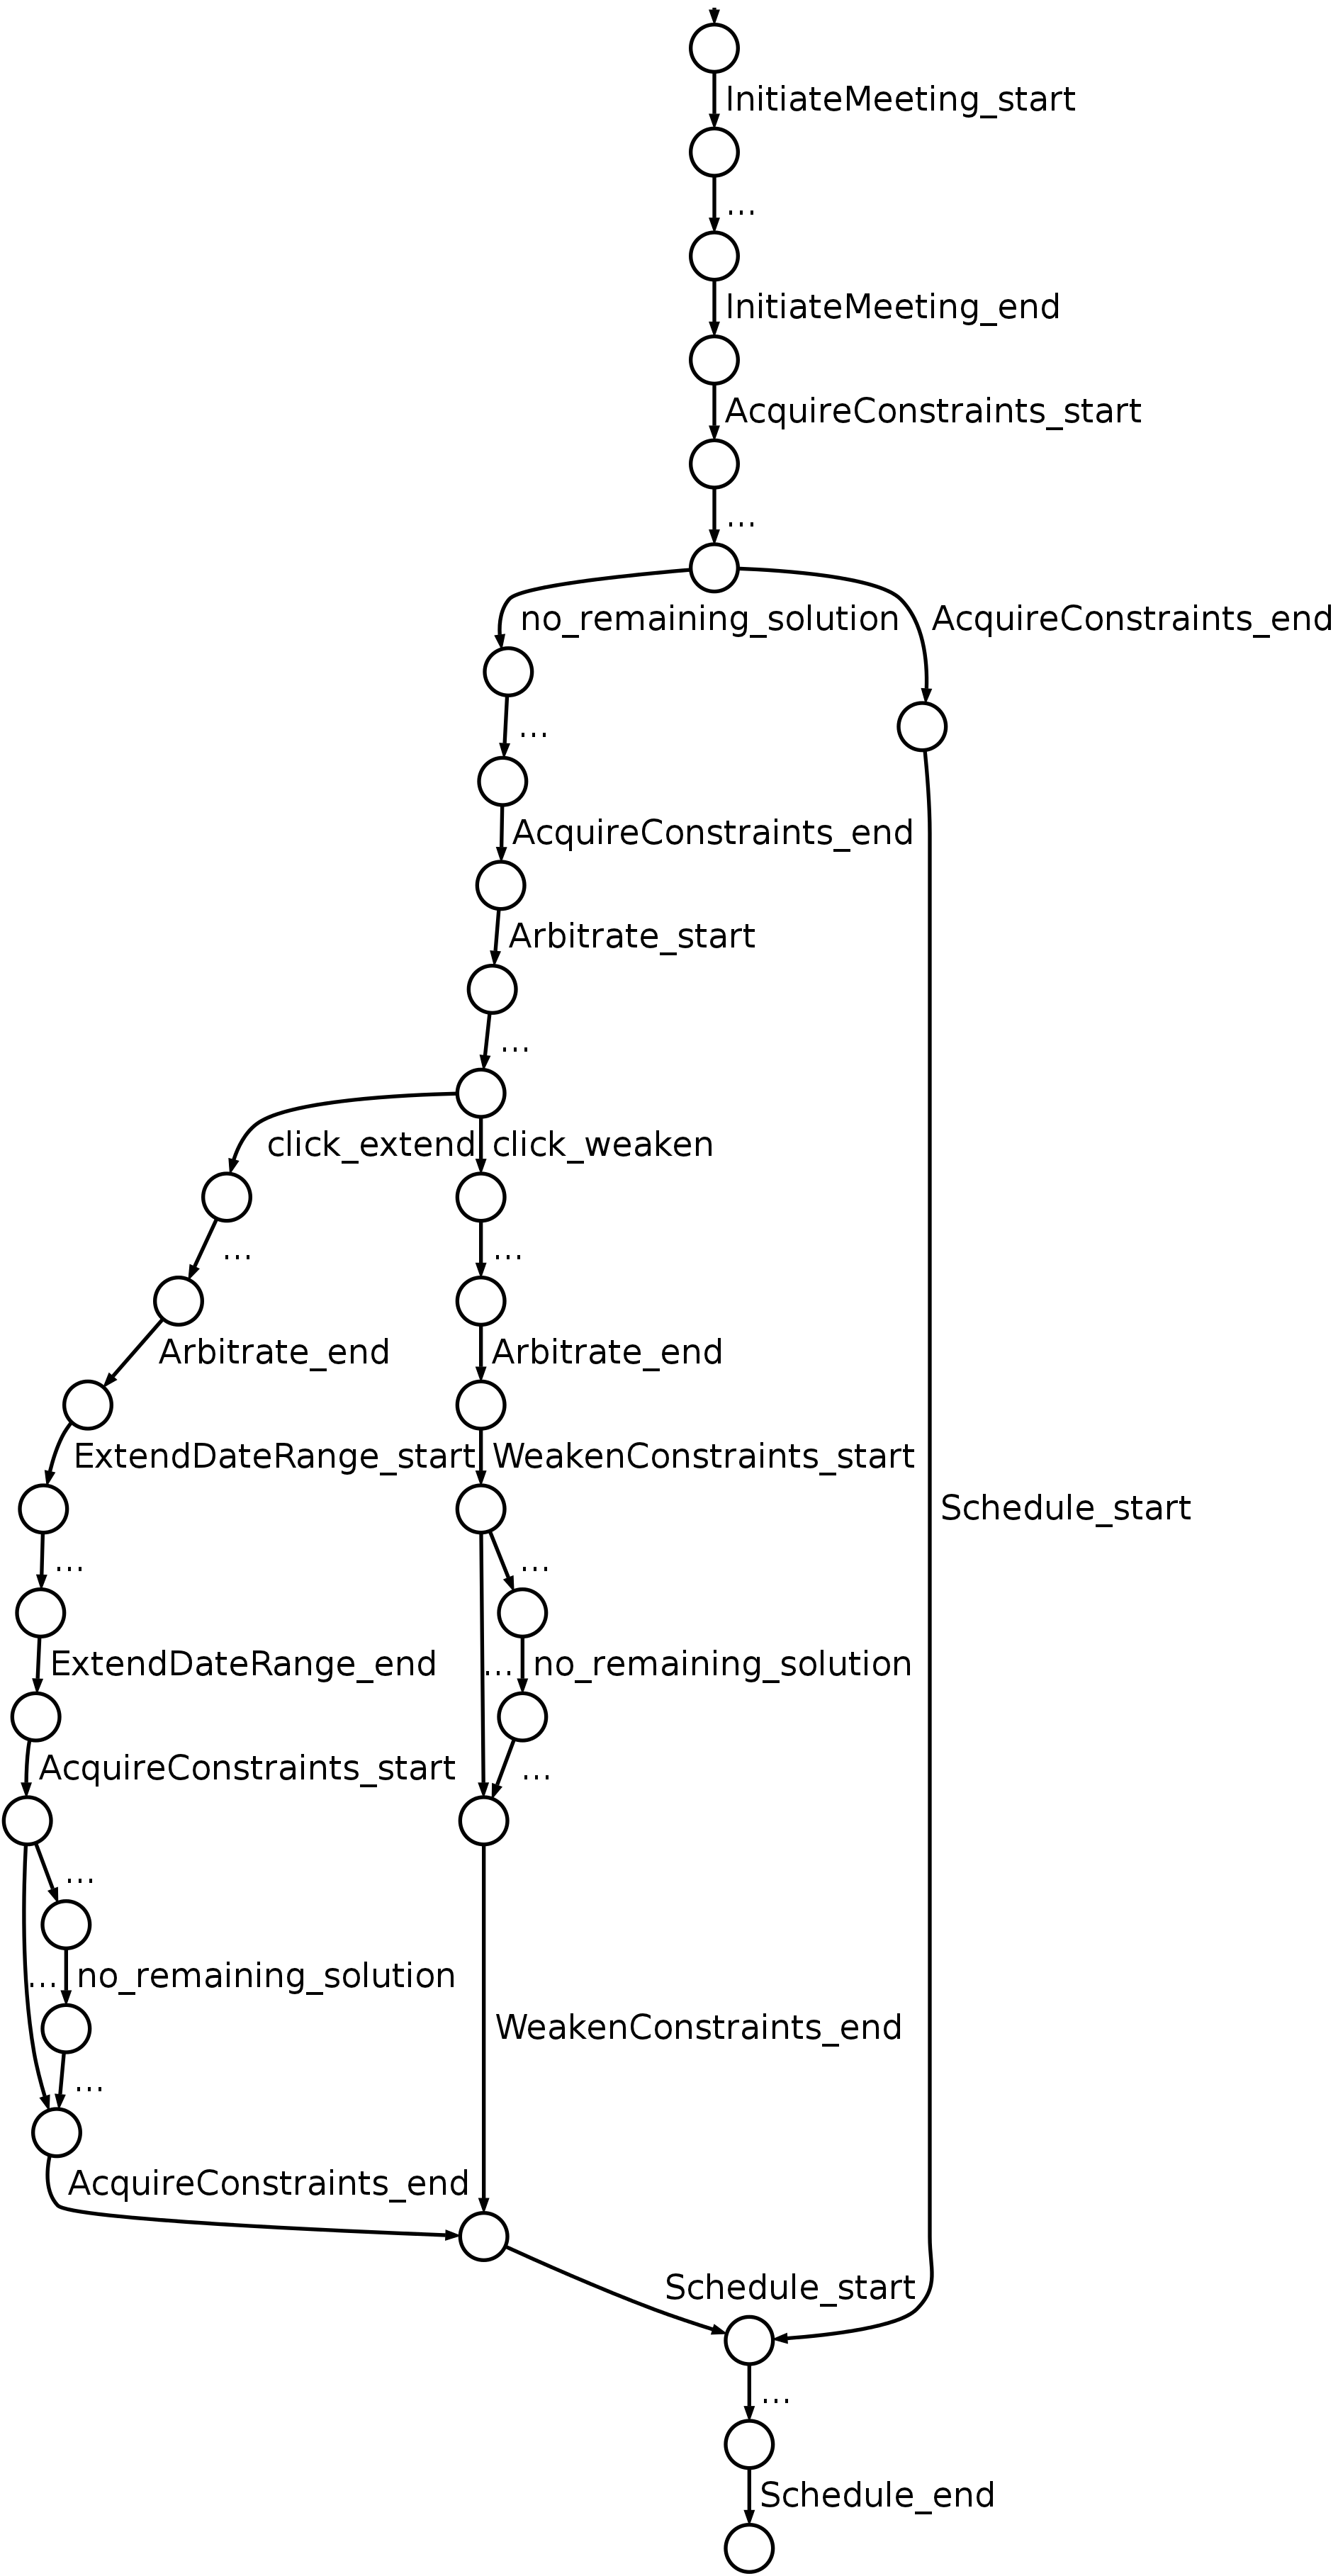
\includegraphics[trim=2mm 2mm 2mm 2mm, clip]{src/3-deductive/images/scheduler-lts}
}
\caption[Trace-equivalent LTS for the meeting scheduling example]{Trace-equivalent LTS for the meeting scheduling example from Fig.~\ref{image:scheduler-ghmsc}.\label{image:scheduler-lts}}
\end{figure}

\subsubsection*{A note on temporal complexity}

By construction, our composition technique always considers $2^{\mid\Phi\mid}$ initial fluent assignments, pruning those that do not satisfy $C_0$. In practice, certain fluents have a specific initial value; in this case, the corresponding fluent automaton can be optimized by removing a transition from its initial state. This allows avoiding to compute some of the unsatisfiable conjunctions on the compound initial state. 

The approach might even be improved so as to consider only fluent initializations satisfying $C_0$. If such optimization speeds up the computation in practice, the exponential blow of the resulting trace LTS remains unavoidable. It naturally results from the ability of models with guards to cover numerous behaviors in an implicit, compact way.


